% ============================================================
% 第19章 一次函数 — 人教版八年级下册讲义
% 编译命令：xelatex -interaction=nonstopmode 第19章_一次函数.tex
% ============================================================
\documentclass[12pt, a4paper]{ctexart}
\usepackage[margin=2.2cm]{geometry}
\usepackage{amsmath, amssymb}
\usepackage{enumitem}
\usepackage{tcolorbox}
\usepackage{booktabs}
\usepackage{array}
\usepackage{fancyhdr}
\usepackage{xcolor}
\usepackage{tikz}
\usepackage{hyperref}
\usepackage{graphicx}
\usepackage{multirow}
\usepackage{pgfplots}
\pgfplotsset{compat=1.18}

% 颜色定义
\definecolor{mainblue}{RGB}{41, 98, 168}
\definecolor{lightblue}{RGB}{230, 240, 255}
\definecolor{tipgreen}{RGB}{34, 139, 87}
\definecolor{lightgreen}{RGB}{235, 250, 240}
\definecolor{warnred}{RGB}{200, 50, 50}
\definecolor{lightred}{RGB}{255, 240, 240}
\definecolor{examorange}{RGB}{210, 120, 20}
\definecolor{lightorange}{RGB}{255, 248, 235}
\definecolor{apppurple}{RGB}{120, 60, 170}
\definecolor{lightpurple}{RGB}{245, 238, 255}

% 页眉页脚
\pagestyle{fancy}
\fancyhf{}
\fancyhead[L]{\small\textcolor{mainblue}{\textbf{人教版八年级下册 · 第19章 一次函数}}}
\fancyhead[R]{\small\textcolor{mainblue}{家教讲义}}
\fancyfoot[C]{\small —\ \thepage\ —}
\renewcommand{\headrulewidth}{0.6pt}
\renewcommand{\headrule}{\hbox to\headwidth{\color{mainblue}\leaders\hrule height \headrulewidth\hfill}}
\renewcommand{\footrulewidth}{0pt}

% tcolorbox 样式
\newtcolorbox{knowledgebox}[1][]{%
  colback=lightblue, colframe=mainblue,
  fonttitle=\bfseries\large, title=#1,
  arc=3mm, boxrule=0.8pt,
  left=8pt, right=8pt, top=6pt, bottom=6pt
}

\newtcolorbox{tipbox}[1][]{%
  colback=lightgreen, colframe=tipgreen,
  fonttitle=\bfseries, title=#1,
  arc=2mm, boxrule=0.6pt,
  left=6pt, right=6pt, top=4pt, bottom=4pt
}

\newtcolorbox{warnbox}[1][]{%
  colback=lightred, colframe=warnred,
  fonttitle=\bfseries, title=#1,
  arc=2mm, boxrule=0.6pt,
  left=6pt, right=6pt, top=4pt, bottom=4pt
}

\newtcolorbox{examplebox}[1][]{%
  colback=lightorange, colframe=examorange,
  fonttitle=\bfseries, title=#1,
  arc=3mm, boxrule=0.8pt,
  left=8pt, right=8pt, top=6pt, bottom=6pt
}

\newtcolorbox{appbox}[1][]{%
  colback=lightpurple, colframe=apppurple,
  fonttitle=\bfseries, title=#1,
  arc=3mm, boxrule=0.8pt,
  left=8pt, right=8pt, top=6pt, bottom=6pt
}

\setCJKmainfont{Hiragino Sans GB}
\setCJKsansfont{Heiti SC}

\begin{document}

% ============ 标题页 ============
\begin{center}
{\Huge\bfseries\textcolor{mainblue}{第19章\quad 一次函数}}\\[12pt]
{\Large\textcolor{gray}{讲\quad 义}}\\[8pt]
\rule{0.6\textwidth}{1pt}\\[8pt]
{\normalsize 适用：人教版\quad 八年级下册\quad |\quad 课时：6课时}
\end{center}
\vspace{10pt}

% ============================================================
%  第一部分：知识点讲解
% ============================================================
\section*{\textcolor{mainblue}{一、知识点讲解}}

\subsection*{19.1\quad 变量与函数}

\begin{knowledgebox}[变量与常量]
在一个变化过程中，数值\textbf{发生变化}的量叫做\textbf{变量}，数值\textbf{始终不变}的量叫做\textbf{常量}。

例如：在匀速运动 $s = vt$ 中，$s$ 和 $t$ 是变量，$v$ 是常量。
\end{knowledgebox}

\begin{knowledgebox}[函数的定义]
一般地，在一个变化过程中，如果有两个变量 $x$ 与 $y$，并且对于 $x$ 的每一个确定的值，$y$ 都有\textbf{唯一确定}的值与其对应，那么就说 $y$ 是 $x$ 的\textbf{函数}，$x$ 叫做\textbf{自变量}。

\begin{itemize}[leftmargin=2em]
  \item \textbf{自变量的取值范围}：使函数解析式有意义的自变量取值的全体。
  \item 例如 $y=\dfrac{1}{x-2}$ 中，$x\neq 2$；$y=\sqrt{x}$ 中，$x\geqslant 0$。
\end{itemize}
\end{knowledgebox}

\begin{knowledgebox}[函数的三种表示法]
\begin{enumerate}[leftmargin=2em]
  \item \textbf{列表法}：用表格列出 $x$ 与 $y$ 的对应值。
  \item \textbf{解析式法}：用数学式子（解析式）表示 $x$ 与 $y$ 的关系，如 $y=2x+1$。
  \item \textbf{图象法}：用图象（通常是平面直角坐标系中的曲线或直线）表示 $x$ 与 $y$ 的关系。
\end{enumerate}
\end{knowledgebox}

\begin{warnbox}[易错提醒]
\begin{itemize}[leftmargin=2em]
  \item 判断 $y$ 是否是 $x$ 的函数，关键在于"唯一确定"——每个 $x$ 对应的 $y$ 只能有一个。
  \item $y = \pm\sqrt{x}$ \textbf{不是}函数，因为一个 $x$ 对应了两个 $y$ 值。
\end{itemize}
\end{warnbox}

\subsection*{19.2\quad 正比例函数}

\begin{knowledgebox}[正比例函数的定义与图象]
\textbf{定义}：形如 $y = kx$（$k$ 为常数，$k\neq 0$）的函数叫做\textbf{正比例函数}，其中 $k$ 叫做\textbf{比例系数}。

\textbf{图象}：正比例函数 $y=kx$ 的图象是经过原点 $(0,0)$ 和点 $(1,k)$ 的一条\textbf{直线}。

\textbf{性质}：
\begin{itemize}[leftmargin=2em]
  \item 当 $k>0$ 时，直线经过\textbf{第一、三象限}，$y$ 随 $x$ 增大而\textbf{增大}（递增）。
  \item 当 $k<0$ 时，直线经过\textbf{第二、四象限}，$y$ 随 $x$ 增大而\textbf{减小}（递减）。
\end{itemize}
\end{knowledgebox}

正比例函数 $y = 2x$ 与 $y = -2x$ 的图象对比如下：

\begin{center}
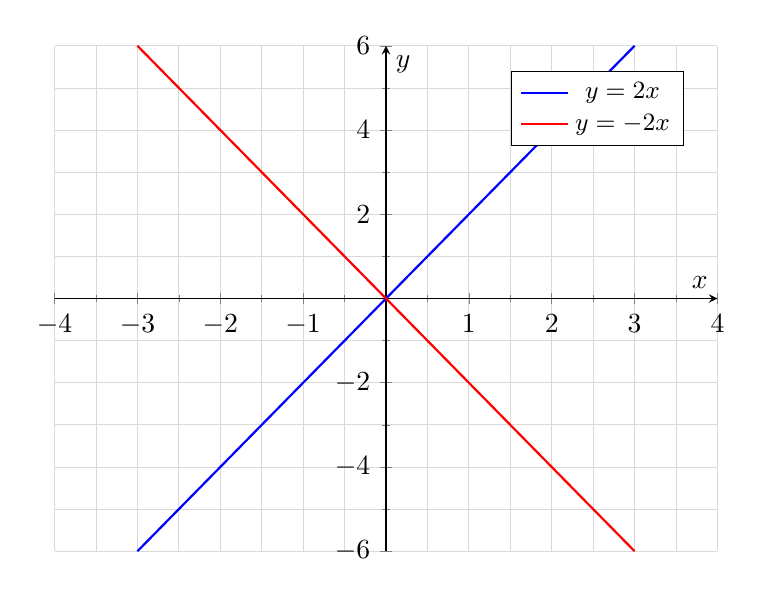
\begin{tikzpicture}
\begin{axis}[
    width=10cm, height=8cm,
    axis lines=middle,
    xlabel=$x$, ylabel=$y$,
    xmin=-4, xmax=4, ymin=-6, ymax=6,
    grid=both,
    grid style={line width=0.3pt, draw=gray!30},
    minor tick num=1,
    legend style={at={(0.95,0.95)}, anchor=north east, font=\small},
    every axis plot/.append style={thick}
]
\addplot[blue, domain=-3:3] {2*x};
\addlegendentry{$y=2x$}
\addplot[red, domain=-3:3] {-2*x};
\addlegendentry{$y=-2x$}
\end{axis}
\end{tikzpicture}
\end{center}

\subsection*{19.3\quad 一次函数}

\begin{knowledgebox}[一次函数的定义与图象]
\textbf{定义}：形如 $y = kx + b$（$k,b$ 为常数，$k\neq 0$）的函数叫做\textbf{一次函数}。

特别地，当 $b=0$ 时，$y=kx$ 就是正比例函数——正比例函数是一次函数的特殊情况。

\textbf{图象}：一次函数 $y=kx+b$ 的图象是一条直线，可以看作将直线 $y=kx$ 沿 $y$ 轴方向平移 $|b|$ 个单位。
\begin{itemize}[leftmargin=2em]
  \item 直线经过点 $(0, b)$（即 $y$ 轴截距）和点 $\left(-\dfrac{b}{k},\ 0\right)$（即 $x$ 轴截距）。
\end{itemize}
\end{knowledgebox}

\begin{knowledgebox}[一次函数的性质——$k$、$b$ 与图象]
\begin{center}
\renewcommand{\arraystretch}{1.4}
\begin{tabular}{|c|c|l|}
\hline
\textbf{$k$ 的符号} & \textbf{$b$ 的符号} & \textbf{图象特征} \\
\hline
$k>0$ & $b>0$ & 经过第一、二、三象限，递增 \\
\hline
$k>0$ & $b<0$ & 经过第一、三、四象限，递增 \\
\hline
$k<0$ & $b>0$ & 经过第一、二、四象限，递减 \\
\hline
$k<0$ & $b<0$ & 经过第二、三、四象限，递减 \\
\hline
\end{tabular}
\end{center}
\end{knowledgebox}

下面是四种情况的图象：

\begin{center}
\begin{tikzpicture}
% k>0, b>0
\begin{axis}[
    width=6cm, height=5.5cm,
    at={(0,0)}, anchor=origin,
    axis lines=middle, xlabel=$x$, ylabel=$y$,
    xmin=-3, xmax=3, ymin=-3, ymax=5,
    grid=both, grid style={line width=0.2pt, draw=gray!30},
    title={\small $k>0,\ b>0$}, title style={at={(0.5,1.05)}},
    every axis plot/.append style={thick},
    xtick=\empty, ytick=\empty
]
\addplot[blue, domain=-2.5:2.5] {x+2};
\end{axis}

% k>0, b<0
\begin{axis}[
    width=6cm, height=5.5cm,
    at={(7cm,0)}, anchor=origin,
    axis lines=middle, xlabel=$x$, ylabel=$y$,
    xmin=-3, xmax=3, ymin=-5, ymax=3,
    grid=both, grid style={line width=0.2pt, draw=gray!30},
    title={\small $k>0,\ b<0$}, title style={at={(0.5,1.05)}},
    every axis plot/.append style={thick},
    xtick=\empty, ytick=\empty
]
\addplot[blue, domain=-0.5:2.5] {x-2};
\end{axis}

% k<0, b>0
\begin{axis}[
    width=6cm, height=5.5cm,
    at={(0,-7cm)}, anchor=origin,
    axis lines=middle, xlabel=$x$, ylabel=$y$,
    xmin=-3, xmax=3, ymin=-3, ymax=5,
    grid=both, grid style={line width=0.2pt, draw=gray!30},
    title={\small $k<0,\ b>0$}, title style={at={(0.5,1.05)}},
    every axis plot/.append style={thick},
    xtick=\empty, ytick=\empty
]
\addplot[red, domain=-1:2.5] {-x+2};
\end{axis}

% k<0, b<0
\begin{axis}[
    width=6cm, height=5.5cm,
    at={(7cm,-7cm)}, anchor=origin,
    axis lines=middle, xlabel=$x$, ylabel=$y$,
    xmin=-3, xmax=3, ymin=-5, ymax=3,
    grid=both, grid style={line width=0.2pt, draw=gray!30},
    title={\small $k<0,\ b<0$}, title style={at={(0.5,1.05)}},
    every axis plot/.append style={thick},
    xtick=\empty, ytick=\empty
]
\addplot[red, domain=-2.5:1] {-x-2};
\end{axis}
\end{tikzpicture}
\end{center}

\begin{tipbox}[快速判断技巧]
\textbf{看 $k$ 定升降}：$k>0$ 则 $y$ 随 $x$ 增大而增大（从左下到右上）；$k<0$ 则相反。

\textbf{看 $b$ 定交点}：$b>0$ 直线交 $y$ 轴正半轴；$b<0$ 交 $y$ 轴负半轴；$b=0$ 过原点。
\end{tipbox}

\subsection*{19.4\quad 用待定系数法求一次函数解析式}

\begin{knowledgebox}[待定系数法]
如果已知 $y$ 是 $x$ 的一次函数，即 $y = kx + b$（$k\neq 0$），那么只需知道直线上\textbf{两个点}的坐标，就可以确定 $k$ 和 $b$ 的值。

\textbf{步骤}：
\begin{enumerate}[leftmargin=2em]
  \item 设函数解析式为 $y = kx + b$（$k\neq 0$）。
  \item 将已知的两组 $(x, y)$ 代入，得到关于 $k$、$b$ 的二元一次方程组。
  \item 解方程组，求出 $k$、$b$。
  \item 写出解析式。
\end{enumerate}
\end{knowledgebox}

\subsection*{19.5\quad 一次函数与方程、不等式的关系}

\begin{knowledgebox}[一次函数与一元一次方程]
求一元一次方程 $kx + b = 0$（$k\neq 0$）的解，等价于求一次函数 $y = kx + b$ 的图象与 $x$ 轴交点的\textbf{横坐标}。

\medskip
\textbf{一般地}：对于一次函数 $y = kx + b$，令 $y = 0$，得 $kx + b = 0$，解为 $x = -\dfrac{b}{k}$。
\end{knowledgebox}

\begin{knowledgebox}[一次函数与一元一次不等式]
\begin{itemize}[leftmargin=2em]
  \item $kx + b > 0$ 的解集 $\Longleftrightarrow$ 一次函数 $y = kx + b$ 的图象在 $x$ 轴\textbf{上方}对应的 $x$ 的范围。
  \item $kx + b < 0$ 的解集 $\Longleftrightarrow$ 一次函数 $y = kx + b$ 的图象在 $x$ 轴\textbf{下方}对应的 $x$ 的范围。
\end{itemize}

例如：若直线 $y = 2x - 4$，则 $2x - 4 > 0$ 的解集为 $x > 2$。
\end{knowledgebox}

\subsection*{19.6\quad 两直线的位置关系}

\begin{knowledgebox}[两条直线的位置关系]
设直线 $l_1: y = k_1 x + b_1$，$l_2: y = k_2 x + b_2$，则：
\begin{itemize}[leftmargin=2em]
  \item $k_1 = k_2$ 且 $b_1 \neq b_2$ $\Longleftrightarrow$ 两直线\textbf{平行}。
  \item $k_1 \neq k_2$ $\Longleftrightarrow$ 两直线\textbf{相交}。
  \item $k_1 = k_2$ 且 $b_1 = b_2$ $\Longleftrightarrow$ 两直线\textbf{重合}。
\end{itemize}
\end{knowledgebox}

\begin{warnbox}[易错提醒]
两直线平行的条件是 $k$ 相同且 $b$ 不同，不能只看 $k$ 相同就判断平行——还要确认 $b$ 不同。
\end{warnbox}

% ============================================================
%  第二部分：例题精讲
% ============================================================
\section*{\textcolor{examorange}{二、例题精讲}}

\begin{examplebox}[【例题1】基础概念——判断函数关系]
下列关系式中，$y$ 是 $x$ 的函数的是\quad（\quad）

A. $y^2 = x$ \quad B. $y = \pm\sqrt{x}$ \quad C. $|y| = x$ \quad D. $y = \dfrac{1}{x+1}$
\end{examplebox}

\textbf{解}：

A. $y^2 = x$，当 $x = 4$ 时，$y = 2$ 或 $y = -2$，一个 $x$ 对应两个 $y$，不是函数。

B. $y = \pm\sqrt{x}$ 同理，一个 $x$ 对应两个 $y$，不是函数。

C. $|y| = x$，当 $x = 1$ 时，$y = 1$ 或 $y = -1$，不是函数。

D. $y = \dfrac{1}{x+1}$，每个 $x\neq -1$ 对应唯一确定的 $y$，是函数。

\textbf{答案}：D。

\begin{tipbox}[方法总结]
判断是否为函数，核心标准是"对于 $x$ 的每一个值，$y$ 是否唯一确定"。如果一个 $x$ 对应多个 $y$，就不是函数。
\end{tipbox}

\begin{examplebox}[【例题2】正比例函数的图象与性质]
已知正比例函数 $y = (m-1)x^{m^2-3}$ 的图象经过第二、四象限，求 $m$ 的值。
\end{examplebox}

\textbf{解}：

因为 $y = (m-1)x^{m^2-3}$ 是正比例函数，所以自变量 $x$ 的指数必须为 $1$：
$$m^2 - 3 = 1 \implies m^2 = 4 \implies m = 2 \text{ 或 } m = -2$$

又因为图象经过第二、四象限，所以 $k = m - 1 < 0$，即 $m < 1$。

因此 $m = 2$（不满足 $m<1$，舍去），$m = -2$（满足 $m < 1$）。

当 $m = -2$ 时，$k = m - 1 = -3$，$y = -3x$，经过第二、四象限。$\checkmark$

\textbf{答案}：$m = -2$。

\begin{tipbox}[方法总结]
正比例函数 $y = kx$ 中：(1) $x$ 的指数必须恰好为 $1$；(2) $k \neq 0$；(3) 利用图象所在象限判断 $k$ 的符号。
\end{tipbox}

\begin{examplebox}[【例题3】一次函数图象过象限问题]
已知一次函数 $y = (2a+4)x - (3-b)$，当 $a$、$b$ 为何值时：
\begin{enumerate}[leftmargin=2em]
  \item $y$ 随 $x$ 增大而增大；
  \item 图象经过第一、二、三象限；
  \item 图象与 $y$ 轴的交点在 $x$ 轴上方。
\end{enumerate}
\end{examplebox}

\textbf{解}：

设 $k = 2a + 4$，$b_0 = -(3-b) = b - 3$。

\begin{enumerate}[leftmargin=2em]
  \item $y$ 随 $x$ 增大而增大 $\Longleftrightarrow$ $k > 0$，即 $2a + 4 > 0$，解得 $a > -2$。
  \item 图象经过第一、二、三象限 $\Longleftrightarrow$ $k > 0$ 且 $b_0 > 0$，即 $a > -2$ 且 $b > 3$。
  \item 图象与 $y$ 轴的交点在 $x$ 轴上方 $\Longleftrightarrow$ $b_0 > 0$，即 $b > 3$。
\end{enumerate}

\begin{tipbox}[方法总结]
一次函数 $y = kx + b$ 中：
\begin{itemize}[leftmargin=2em]
  \item $k$ 决定升降（$k>0$ 递增，$k<0$ 递减）；
  \item $b$ 决定与 $y$ 轴交点位置（$b>0$ 在上方，$b<0$ 在下方）；
  \item 两者共同决定图象经过的象限。
\end{itemize}
\end{tipbox}

\begin{examplebox}[【例题4】用待定系数法求解析式]
已知一次函数的图象经过点 $A(1, 3)$ 和点 $B(-1, -1)$，求这个一次函数的解析式。
\end{examplebox}

\textbf{解}：

设一次函数解析式为 $y = kx + b$（$k\neq 0$）。

将 $A(1,3)$ 和 $B(-1,-1)$ 代入：
$$\begin{cases} k \cdot 1 + b = 3 \\ k \cdot (-1) + b = -1 \end{cases} \implies \begin{cases} k + b = 3 \\ -k + b = -1 \end{cases}$$

两式相减：$2k = 4$，解得 $k = 2$。

代入第一式：$2 + b = 3$，解得 $b = 1$。

\textbf{答案}：$y = 2x + 1$。

\begin{tipbox}[方法总结]
待定系数法的核心：设解析式 $\to$ 代入已知点 $\to$ 解方程组。两个未知数（$k$、$b$）需要两个方程，即两个点的坐标。
\end{tipbox}

\begin{examplebox}[【例题5】一次函数与不等式的综合]
如图，直线 $y = kx + b$ 经过点 $A(-2, 4)$ 和点 $B(1, -2)$。

\begin{enumerate}[leftmargin=2em]
  \item 求直线的解析式；
  \item 根据图象，直接写出 $kx + b > 0$ 的解集。
\end{enumerate}

\begin{center}
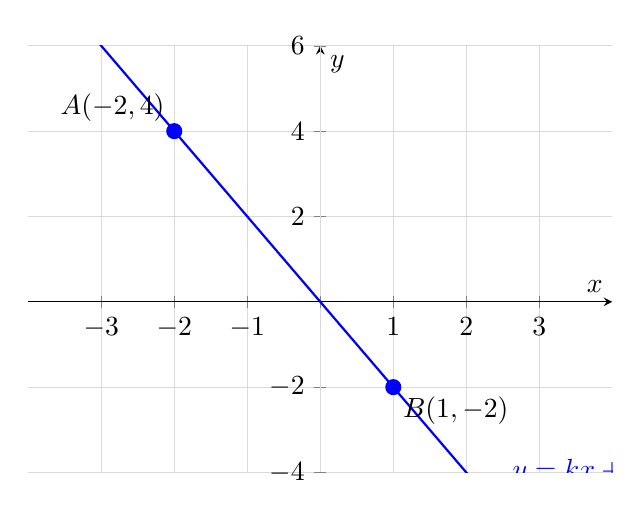
\begin{tikzpicture}
\begin{axis}[
    width=9cm, height=7cm,
    axis lines=middle,
    xlabel=$x$, ylabel=$y$,
    xmin=-4, xmax=4, ymin=-4, ymax=6,
    grid=both,
    grid style={line width=0.3pt, draw=gray!30},
    every axis plot/.append style={thick},
    xtick={-3,-2,-1,0,1,2,3},
    ytick={-4,-2,0,2,4,6},
    extra x ticks={0}, extra x tick labels={}
]
\addplot[blue, domain=-3.5:3] {-2*x};
\node[blue, above right] at (axis cs: 2.5, -4.5) {$y = kx+b$};
\addplot[only marks, mark=*, mark size=2.5pt, blue] coordinates {(-2,4) (1,-2)};
\node[above left] at (axis cs: -2, 4) {$A(-2,4)$};
\node[below right] at (axis cs: 1, -2) {$B(1,-2)$};
\end{axis}
\end{tikzpicture}
\end{center}
\end{examplebox}

\textbf{解}：

\begin{enumerate}[leftmargin=2em]
  \item 将 $A(-2,4)$、$B(1,-2)$ 代入 $y = kx + b$：
  $$\begin{cases} -2k + b = 4 \\ k + b = -2 \end{cases}$$
  第一式减第二式：$-3k = 6$，得 $k = -2$。代入：$-2 + b = -2$，得 $b = 0$。

  所以 $y = -2x$。

  \item 由图象可知，直线 $y = -2x$ 与 $x$ 轴交于原点。当 $x < 0$ 时，$y = -2x > 0$。

  所以 $kx + b > 0$ 即 $-2x > 0$ 的解集为 $x < 0$。
\end{enumerate}

\begin{tipbox}[方法总结]
利用图象解不等式 $kx+b > 0$：找到直线与 $x$ 轴的交点横坐标 $x_0$，观察图象在 $x$ 轴上方的部分对应的 $x$ 范围即为解集。若 $k<0$，则 $x < x_0$；若 $k>0$，则 $x > x_0$。
\end{tipbox}

\begin{examplebox}[【例题6】两直线交点与几何面积综合]
已知直线 $l_1: y = 2x + 1$ 和直线 $l_2: y = -x + 4$。

\begin{enumerate}[leftmargin=2em]
  \item 求两直线的交点坐标；
  \item 求两直线与 $x$ 轴围成的三角形的面积。
\end{enumerate}
\end{examplebox}

\textbf{解}：

\begin{enumerate}[leftmargin=2em]
  \item 联立方程组：
  $$\begin{cases} y = 2x + 1 \\ y = -x + 4 \end{cases}$$
  得 $2x + 1 = -x + 4$，$3x = 3$，$x = 1$，$y = 2 \times 1 + 1 = 3$。

  交点坐标为 $(1, 3)$。

  \item $l_1$ 与 $x$ 轴的交点：令 $y = 0$，$2x + 1 = 0$，$x = -\dfrac{1}{2}$，交点 $C\left(-\dfrac{1}{2}, 0\right)$。

  $l_2$ 与 $x$ 轴的交点：令 $y = 0$，$-x + 4 = 0$，$x = 4$，交点 $D(4, 0)$。

  两直线与 $x$ 轴围成三角形的三个顶点为 $C\left(-\dfrac{1}{2}, 0\right)$、$D(4, 0)$、$P(1, 3)$。

  底边 $CD = 4 - \left(-\dfrac{1}{2}\right) = \dfrac{9}{2}$，高为点 $P$ 到 $x$ 轴的距离 $= 3$。

  $$S = \frac{1}{2} \times \frac{9}{2} \times 3 = \frac{27}{4}$$
\end{enumerate}

\textbf{答案}：交点 $(1, 3)$，面积 $\dfrac{27}{4}$。

\begin{tipbox}[方法总结]
求两直线交点 $\to$ 联立解方程组；求面积 $\to$ 找底和高，注意底边在坐标轴上时，高就是第三个顶点到坐标轴的距离。一次函数与几何图形的综合题是中考热点。
\end{tipbox}

\begin{examplebox}[【例题7】读图题——从图象获取信息]
小明从家出发骑自行车去图书馆，途中休息了一段时间后继续骑行到达图书馆。以下哪幅图最能反映小明离家的距离 $s$ 与时间 $t$ 的关系？

\begin{center}
\begin{tikzpicture}
\begin{axis}[
    width=11cm, height=5cm,
    axis lines=left,
    xlabel={\small 时间 $t$}, ylabel={\small 距离 $s$},
    xmin=0, xmax=6, ymin=0, ymax=5,
    xtick=\empty, ytick=\empty,
    every axis plot/.append style={thick},
    legend style={at={(0.02,0.98)}, anchor=north west, font=\small}
]
\addplot[blue, domain=0:1] {3*x};
\addplot[blue, domain=1:2] {3};
\addplot[blue, domain=2:4] {3+1.5*(x-2)};
\addlegendentry{图 A（先快后慢再平）}

\addplot[red, domain=0:2, dashed] {2*x};
\addplot[red, domain=2:3, dashed] {4};
\addplot[red, domain=3:5, dashed] {4+0.5*(x-3)};
\addlegendentry{图 B（先匀速后休息再匀速）}
\end{axis}
\end{tikzpicture}
\end{center}

图 B 中，出发阶段斜率较大（骑得快），中间有一段水平线（休息，距离不变），最后斜率较小（骑得慢一些），到达图书馆后距离不再变化。请指出哪幅图最合理，并说明理由。
\end{examplebox}

\textbf{解}：

图 B 最合理。

理由：
\begin{itemize}[leftmargin=2em]
  \item 第一阶段（$0 \to 2$）：斜率较大，表示骑行速度较快；
  \item 第二阶段（$2 \to 3$）：斜率为 $0$（水平线段），表示距离不变，即小明在休息；
  \item 第三阶段（$3 \to 5$）：斜率较小但仍为正，表示继续骑行但速度较慢；
  \item 最终到达图书馆，距离保持不变。
\end{itemize}

\begin{tipbox}[方法总结]
读图题要点：(1) 斜率代表变化快慢（速度/效率）；(2) 水平线段代表量不变（休息、停留）；(3) 图象终点的高度代表最终结果。关键是将实际情境与图象特征一一对应。
\end{tipbox}

% ============================================================
%  第三部分：应用题
% ============================================================
\section*{\textcolor{apppurple}{三、应用题}}

\begin{appbox}[【应用1】出租车计费问题]
某市出租车收费标准如下：起步价 $8$ 元（$3$ 千米以内），超过 $3$ 千米后每千米加收 $2$ 元（不足 $1$ 千米按 $1$ 千米计算）。

\begin{enumerate}[leftmargin=2em]
  \item 写出行驶 $x$ 千米（$x>3$ 且 $x$ 为整数）时，车费 $y$（元）与行驶路程 $x$（千米）之间的函数关系式。
  \item 小明乘坐出租车行驶了 $10$ 千米，应付多少元？
\end{enumerate}
\end{appbox}

\textbf{解}：

\begin{enumerate}[leftmargin=2em]
  \item 当 $x > 3$（$x$ 为整数）时：
  $$y = 8 + 2(x - 3) = 2x + 2 \quad (x > 3,\ x \text{为整数})$$

  \item 当 $x = 10$ 时：$y = 2 \times 10 + 2 = 22$（元）。
\end{enumerate}

\textbf{答案}：$y = 2x + 2$（$x>3$），行驶 $10$ 千米应付 $22$ 元。

\begin{appbox}[【应用2】手机套餐选择问题]
甲、乙两家手机通讯公司提供不同的月租套餐：

\begin{itemize}[leftmargin=2em]
  \item \textbf{甲公司}：月租 $30$ 元，通话每分钟 $0.1$ 元。
  \item \textbf{乙公司}：无月租，通话每分钟 $0.3$ 元。
\end{itemize}

\begin{enumerate}[leftmargin=2em]
  \item 分别写出两家公司的月费用 $y$（元）与通话时间 $x$（分钟）之间的函数关系式。
  \item 每月通话多少分钟时，两家公司的费用相同？
  \item 若小华每月通话约 $200$ 分钟，选择哪家公司更合算？
\end{enumerate}
\end{appbox}

\textbf{解}：

\begin{enumerate}[leftmargin=2em]
  \item 甲公司：$y_1 = 0.1x + 30$；\quad 乙公司：$y_2 = 0.3x$。

  \item 令 $y_1 = y_2$：$0.1x + 30 = 0.3x$，$0.2x = 30$，$x = 150$。

  每月通话 $150$ 分钟时，两家费用相同（均为 $45$ 元）。

  \item 当 $x = 200$ 时：$y_1 = 0.1 \times 200 + 30 = 50$（元），$y_2 = 0.3 \times 200 = 60$（元）。

  $50 < 60$，选择\textbf{甲公司}更合算。
\end{enumerate}

\begin{appbox}[【应用3】行程问题——两人相遇]
甲、乙两地相距 $120$ 千米。小明从甲地出发以 $20$ 千米/时的速度骑自行车前往乙地；$1$ 小时后，小红从乙地出发以 $40$ 千米/时的速度骑自行车前往甲地。

\begin{enumerate}[leftmargin=2em]
  \item 分别写出小明和小红离甲地的距离 $s$（千米）与出发时间 $t$（小时）的函数关系式（小明出发时 $t=0$）。
  \item 两人何时相遇？相遇时距甲地多远？
\end{enumerate}
\end{appbox}

\textbf{解}：

\begin{enumerate}[leftmargin=2em]
  \item 小明：$s_1 = 20t$（$t \geq 0$）。

  小红在小明出发 $1$ 小时后才出发，她从乙地向甲地行驶，离甲地的距离为：
  $$s_2 = 120 - 40(t - 1) = 160 - 40t \quad (t \geq 1)$$

  \item 令 $s_1 = s_2$：$20t = 160 - 40t$，$60t = 160$，$t = \dfrac{8}{3}$（小时）$= 2$ 小时 $40$ 分钟。

  $s_1 = 20 \times \dfrac{8}{3} = \dfrac{160}{3} \approx 53.3$（千米）。
\end{enumerate}

\textbf{答案}：小明出发 $\dfrac{8}{3}$ 小时后（即 $2$ 小时 $40$ 分钟后）两人相遇，距甲地约 $53.3$ 千米。

% ============================================================
%  第四部分：课堂练习
% ============================================================
\section*{\textcolor{tipgreen}{四、课堂练习}}

\begin{enumerate}[leftmargin=2em]
  \item 函数 $y = \dfrac{\sqrt{x-1}}{x-3}$ 中，自变量 $x$ 的取值范围是\quad（\quad）

  A. $x \geq 1$ \quad B. $x \geq 1$ 且 $x \neq 3$ \quad C. $x > 1$ \quad D. $x \neq 3$

  \item 已知正比例函数 $y = kx$（$k\neq 0$）的图象经过点 $(2, -6)$，则 $k = $ \underline{\qquad}，该函数图象经过第\underline{\qquad}象限。

  \item 一次函数 $y = -3x + 6$ 的图象与 $x$ 轴的交点坐标为\underline{\qquad}，与 $y$ 轴的交点坐标为\underline{\qquad}。

  \item 已知一次函数 $y = kx + b$ 的图象经过 $A(0, -2)$ 和 $B(3, 4)$，求该一次函数的解析式。

  \item 直线 $l_1: y = 2x - 3$ 与直线 $l_2: y = 2x + 1$ 的位置关系是\quad（\quad）

  A. 相交 \quad B. 平行 \quad C. 重合 \quad D. 无法确定
\end{enumerate}

\begin{knowledgebox}[参考答案]
\begin{enumerate}[leftmargin=2em]
  \item \textbf{B}。\quad 要求 $x - 1 \geq 0$ 且 $x - 3 \neq 0$，即 $x \geq 1$ 且 $x \neq 3$。

  \item $k = -3$，经过第\textbf{二、四}象限。\quad 将 $(2, -6)$ 代入 $y = kx$：$-6 = 2k$，$k = -3$。$k<0$ 经过第二、四象限。

  \item 与 $x$ 轴交点 $(2, 0)$，与 $y$ 轴交点 $(0, 6)$。\quad 令 $y=0$：$-3x+6=0$，$x=2$；令 $x=0$：$y=6$。

  \item 将 $A(0,-2)$ 和 $B(3,4)$ 代入 $y = kx + b$：$b = -2$，$3k + (-2) = 4$，$k = 2$。所以 $y = 2x - 2$。

  \item \textbf{B}（平行）。\quad 两直线 $k$ 值相同（$k_1 = k_2 = 2$），但 $b$ 值不同（$-3 \neq 1$），所以平行。
\end{enumerate}
\end{knowledgebox}

\vfill
\begin{center}
\small\textcolor{gray}{本讲义仅供教学参考，例题可根据学生水平调整难度。}
\end{center}

\end{document}
